
\section{Introduction}
\label{sec:introduction}

\begin{figure}
    \centering
    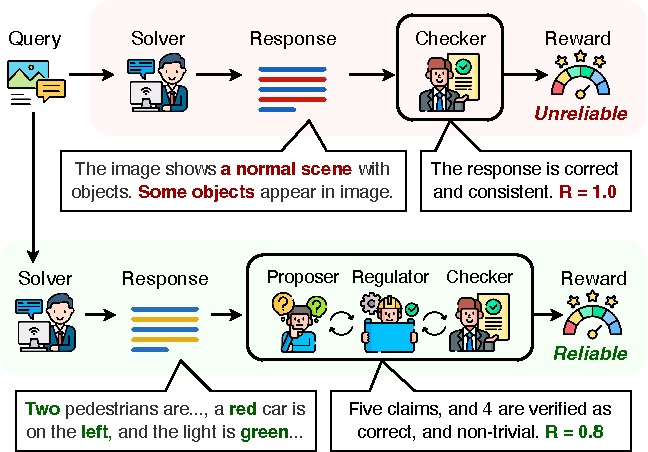
\includegraphics[width=0.98\linewidth]{figures/v-march-intro-final.pdf}
    \caption{\ours achieves reliable visual self-verification rewards through a multi-agent self-check mechanism, encouraging VLMs to generate more informative, image-supported, and diverse responses.
    }
    \label{fig:ours_intro}
    \vspace{-3mm}
\end{figure}

% VLM 的进展和挑战
Vision-Language Models (VLMs) have demonstrated remarkable capabilities across a wide range of multimodal tasks, from image captioning to visual question answering~\cite{achiam2023gpt,touvron2023llama,liu2023llava,chen2024internvl,bai2025qwen3,comanici2025gemini}. 
However, hallucination remains a fundamental bottleneck: models frequently generate descriptions that are fluent and coherent yet factually inconsistent with the visual content of the image~\cite{liu2024survey,rawte2025defining,li2025visual,yang2025mitigating}. 
Such visual hallucinations manifest as fabricated objects, incorrect attributes, or erroneous spatial relationships, and represent a critical barrier to the reliable deployment of VLMs in real-world applications~\cite{dahl2024large,kim2025medical}.
% RLVR 方法存在的挑战
Reinforcement Learning from Verifiable Rewards (RLVR) has emerged as a promising paradigm for improving model factuality 
by optimizing directly against reward signals derived from output correctness
~\cite{shao2024deepseekmath,yu2026dapo,wen2025reinforcement,yue2026does}. 
However, unlike domains such as mathematics or code generation where correctness can be programmatically verified, factual correctness in VLM generation is inherently difficult to verify from images.
% 现有的工作：1.标注/监督 2.self-check/self-play
% TODO: vision-zero, evolmm 还没介绍
Existing approaches to mitigating VLM hallucination largely fall into two categories. 
The first relies on human annotations or external supervision, such as curated factual datasets, preference annotations, or learned reward models~\cite{ouyang2022training,bai2022constitutional}. 
While effective, these methods are expensive to scale and difficult to generalize to large-scale unlabeled image corpora. 
The second category leverages self-checking or self-reflection mechanisms to improve factual consistency through iterative verification or critique~\cite{madaan2023self,shinn2023reflexion,li2026march}. 
% However, existing self-verification approaches are primarily designed for text-only settings and often suffer from confirmation bias when extended to VLMs, since the verifier shares the same hallucination tendencies as the generator. 
However, they lack fine-grained image-grounded verification signals that can reliably assess whether generation is visually supported by the input image, as the verifier can easily rely on textual priors rather than visual evidence, leading to reward hacking and unstable training dynamics (Figure~\ref{fig:ours}).
A key open question remains: 
% \textit{how can we construct a reliable, self-supervised factual verification signal for VLM training, grounded in the image itself, without any human annotation?}
\textbf{\textit{How can VLMs obtain reliable and scalable image-grounded verification signals without relying on annotations or external supervision?}}

\begin{figure}
    \centering
    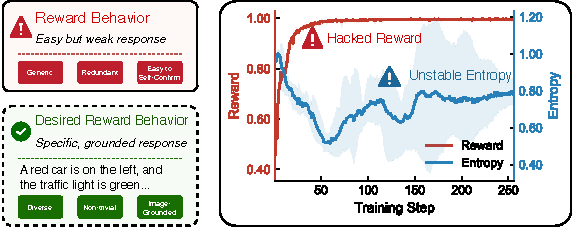
\includegraphics[width=0.98\linewidth]{figures/v-march-motivation-final.pdf}
    \caption{Motivation. Naive self-verification rewards vague but safe descriptions, causing rapid reward growth that reflects reward hacking rather than genuine visual grounding. Reliable visual self-verification should instead favor diverse, non-trivial, and image-grounded claims while maintaining stable training.
    }
    \label{fig:ours}
    \vspace{-3mm}
\end{figure}

To address this, we propose \textbf{\ours}, a visual multi-agent self-check framework for scalable hallucination mitigation in VLMs.
Our insight is that factual verification for VLMs can be approximated through visual regulated self-verification, where generated claims are validated solely against image-grounded visual evidence without accessing the original response~\cite{madaan2023self,li2026march}.
This multi-agent design reduces confirmation bias by decoupling generation from verification, forcing the verifier to rely on the image rather than inherited textual priors~\cite{stechly2025self,jhaveri2026failing}.
% 
Specifically, \ours constructs an automated claim-level multi-agent factual verification pipeline for reinforcement learning. 
% Given a Solver's response, \ours first decomposes it into atomic factual claims through a Proposer agent. Each claim is then transformed into a visual verification question and evaluated by a Checker agent that only observes the input image. 
% The resulting fine-grained verification signals are aggregated into verifiable rewards for RLVR training. 
To further improve the reliability of self-verification rewards, we introduce a Visual Claim Regulation (VCR) mechanism, implemented as a \textbf{Regulator} agent that regularizes the rewards by encouraging informative and image-grounded descriptions while suppressing redundant or weakly supported claims.
% 实验
% We evaluate \ours against nine baselines across 12 benchmarks covering hallucination evaluation, real-world visual question answering, and general multimodal understanding. 
Experimental results across 12 benchmarks show that \ours consistently outperforms existing methods, achieving substantial improvements without relying on ground-truth.
% Additional ablation studies and analyses further demonstrate the effectiveness of the VCR mechanism and the importance of multi-agent design in stabilizing training and improving factuality.
Our main contributions are as follows:
\begin{itemize}
    \setlength{\itemsep}{0pt}
    \setlength{\topsep}{1pt}
    \item We propose \textbf{\ours} method, the first visual multi-agent reinforced self-check framework for VLM hallucination mitigation.
    \item We introduce \textbf{VCR}, a novel mechanism that encourages diverse, informative, and image-grounded descriptions, thereby stabilizing self-verification rewards.
    \item Extensive experiments on 12 benchmarks demonstrate that \ours consistently outperforms existing competitive baselines, establishing a scalable pathway for self-supervised VLM hallucination mitigation.
    \item Comprehensive ablating studies and analyses provide insights into the design of effective self-verification mechanisms for VLMs.
\end{itemize}
